Detta projekt ämnat till att skapa en Ravioli maskin. Raviolin är en traditionell italiensk maträtt bestående av rundor eller kvadratiska pastadeg med fyllning \cite{engproc}. Fyllningen kan bestå av till example köttfärs, skinka och ost. Raviolin serveras ofta i en tomatsås eller köttfärssås. vegetarisk ravioli kan exemplvis fyllas med purjiolök och spenat.\\

Att laga Ravioli hemma har varit jobbigt och tidskrävande. Det tar för mycket tid att fylla på en ravioli deg(utkavlade degen) och resultaten inte blir likadan för alla kuddar.\\

Det finns olika typer av Ravioli maskiner på markanden just nu. En typ av ravioli maskin som visas på figur1, underlättar processen men det mesta görs manuellt.\\

	 		 		\begin{figure}[h]
	 		 			\begin{center}
	 		 				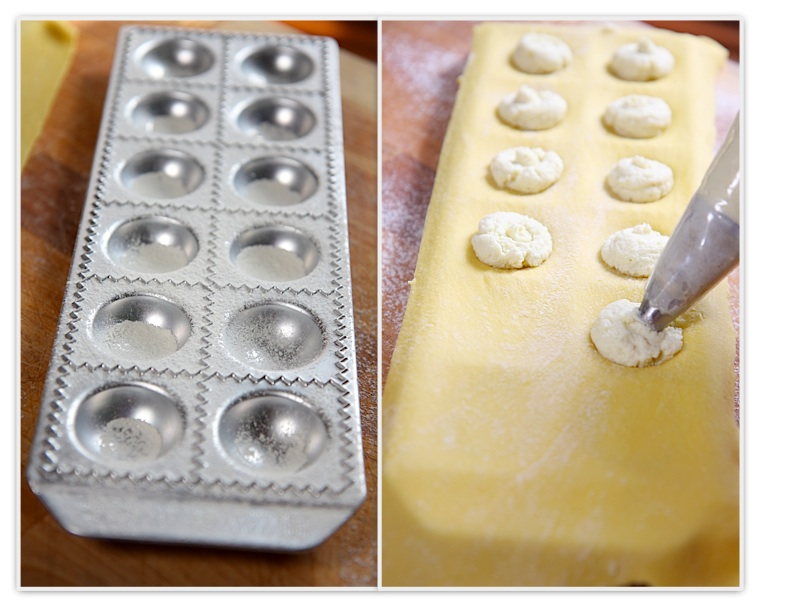
\includegraphics[scale=0.5]{images/raviolimoldwithfilling.jpg}
	 		 				\caption{Raviolimaskin}
	 		 				\label{ravioli}	
	 		 			\end{center}
	 		 		\end{figure}
Den andra typen av maskinen är väldigt stor och priset är högt som medför att de inte kan användas av hushåll, se figur 3. Den typen finns färdig på marknaden.
 		\begin{figure}[h]
 			\begin{center}
 				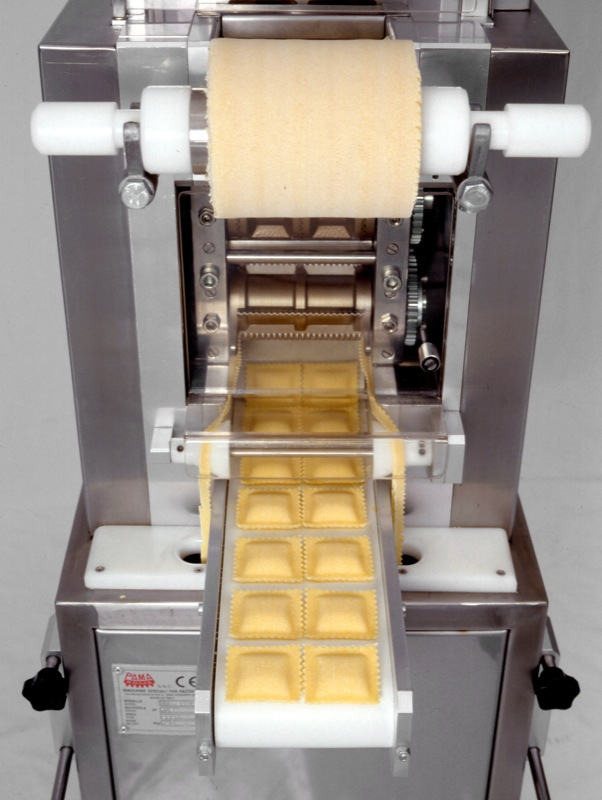
\includegraphics[scale=2]{images/pastamachine.jpg}
 				\caption{Industriell Pasta/Raviolimaskin}
 				\label{pastamaskin}	
 			\end{center}
 		\end{figure}

Idén bakom projektet baseras på behov av en Ravioli maskin och potentiell marknad för den. Tanken är att man utvecklar en liten och bilig Ravioli maskin som kan vara användbar hemma.		